\documentclass[tikz]{standalone}
\usepackage{tikz}
\usepackage{siunitx}
\DeclareSIUnit\degF{\text{°}F}

\definecolor{codeblue}{RGB}{69, 161, 248}
\definecolor{codegray}{RGB}{40, 40, 40}
\usetikzlibrary{shapes,arrows}
\tikzstyle{decision} = [diamond, draw, fill=codegray, text=white,
    text width=4.5em, text badly centered, node distance=3cm, inner sep=0pt]
\tikzstyle{block} = [rectangle, draw, fill=codeblue,  text=white,
    text width=5em, text centered, rounded corners, minimum height=4em]
\tikzstyle{line} = [draw, -latex']


\begin{document}
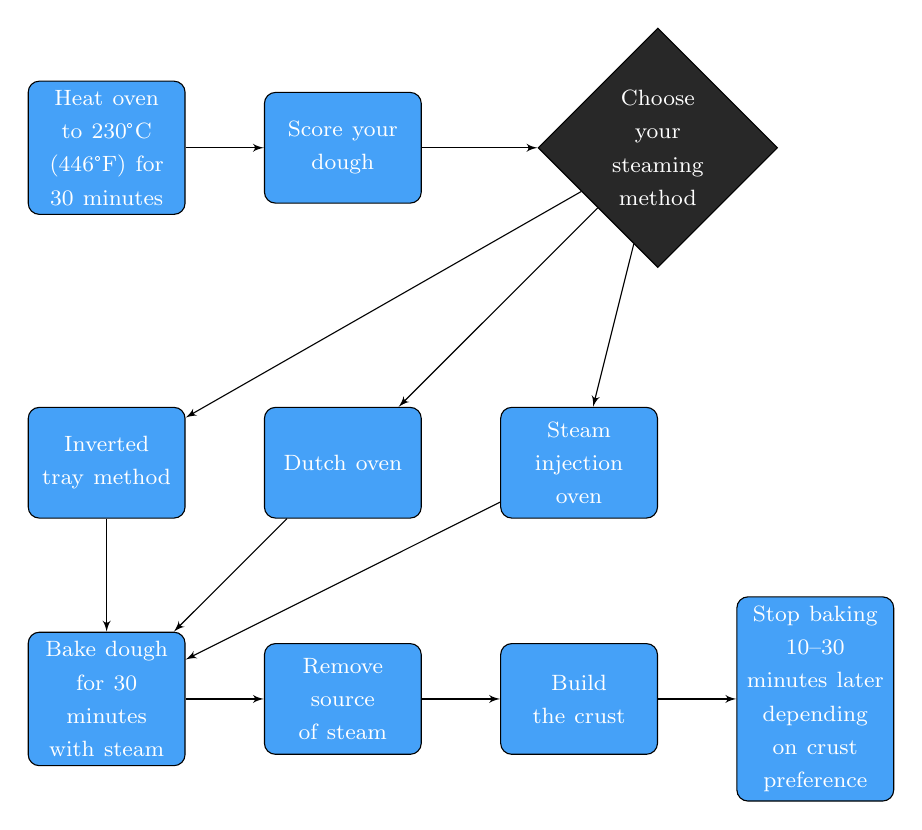
\begin{tikzpicture}[node distance = 3cm, auto]
  \node [block] (heat_oven) {\footnotesize Heat oven to 230°C (446°F) for 30 minutes};
  \node [block, right of=heat_oven, node distance=3cm] (score_dough) {\footnotesize Score your dough};
  \node [decision, right of=score_dough, node distance=4cm] (decide_steam) {\footnotesize Choose your steaming method};
  \node [block, below of=heat_oven, node distance=4cm] (inverted_tray_method) {\footnotesize Inverted tray method};
  \node [block, right of=inverted_tray_method, node distance=3cm] (dutch_oven) {\footnotesize Dutch oven};
  \node [block, right of=dutch_oven, node distance=3cm] (steam_injection) {\footnotesize Steam injection oven};
  \node [block, below of=inverted_tray_method, node distance=3cm] (bake_30) {\footnotesize Bake dough for 30 minutes with steam};
  \node [block, right of=bake_30, node distance=3cm] (remove_steam) {\footnotesize Remove source of steam};
  \node [block, right of=remove_steam, node distance=3cm] (build_crust) {\footnotesize Build the crust};
  \node [block, right of=build_crust, node distance=3cm] (finish_baking) {\footnotesize Stop baking 10--30 minutes later depending on crust preference};
  \path [line] (heat_oven) -- (score_dough);
  \path [line] (score_dough) -- (decide_steam);
  \path [line] (decide_steam) -- (inverted_tray_method);
  \path [line] (decide_steam) -- (dutch_oven);
  \path [line] (decide_steam) -- (steam_injection);
  \path [line] (steam_injection) -- (bake_30);
  \path [line] (inverted_tray_method) -- (bake_30);
  \path [line] (dutch_oven) -- (bake_30);
  \path [line] (bake_30) -- (remove_steam);
  \path [line] (remove_steam) -- (build_crust);
  \path [line] (build_crust) -- (finish_baking);
\end{tikzpicture}
\end{document}
